\documentclass[11pt]{article}
\usepackage{amsmath}

\usepackage{amstext}

\usepackage{amsthm}
\usepackage{color, fullpage, hyperref}
\usepackage{amssymb}
\usepackage{mathtools}
\usepackage{commath}

\usepackage[table]{xcolor}
\usepackage{makecell}

\usepackage{graphicx}
\usepackage{tikz, pgfplots, hf-tikz}
\pgfplotsset{compat=1.17}
\allowdisplaybreaks
\renewcommand\qedsymbol{$\blacksquare$}
\usepackage{tcolorbox}
\tcbuselibrary{theorems}
\tcbuselibrary{fitting}
\usepackage{empheq}

\usepackage[margin=0.5in]{geometry}
\usepackage{fancyvrb}


\title{CSCB07 Lecture 7-9}

%Put assignment number to suit.

\author{Vinesh Benny}

\date{\today}

\begin{document}

\section{SOLID Design}

\begin{itemize}
	\item What is SOLID?
		\begin{itemize}
			\item \textbf{S}ingle Responsibility Principle
			\item \textbf{O}pen/Closed Principle
			\item \textbf{L}iskov Substitution Principle
			\item \textbf{I}nterface Segregation Principle
			\item \textbf{D}ependency Inversion Principle
		\end{itemize}

	\item Single Responsibility Principle (SRP)\\
		\textbf{\emph{A class should have only one reason to change}}
		\begin{itemize}
			\item If you can think of more than one motive for changing a class, then that class has more than one responsibility
			\item If a class has more than one responsibility, then the responsibilities become coupled
			\item Violating the SRP\\
				\begin{center}
					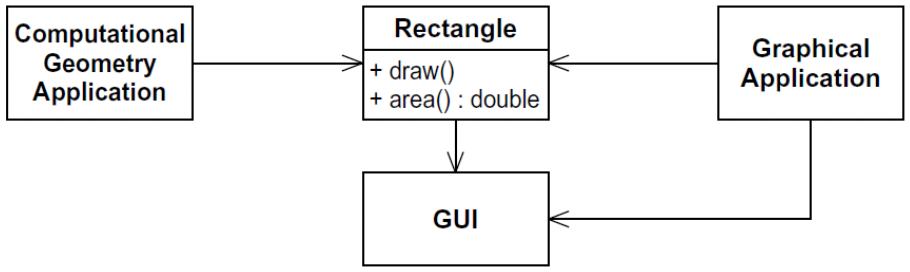
\includegraphics[width=0.6\linewidth]{SRPViolation}
				\end{center}
			\item Conforming to the SRP
				\begin{center}
					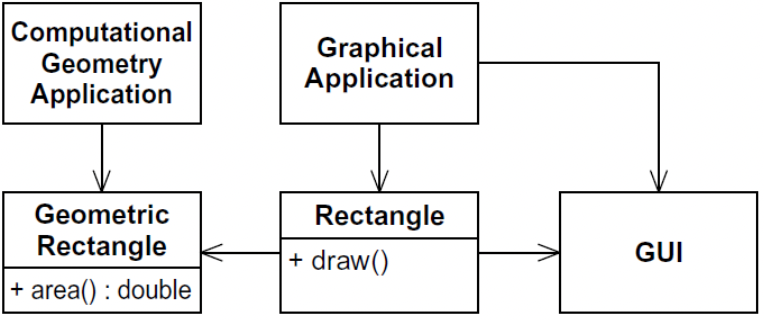
\includegraphics[width=0.5\linewidth]{SRPConform}
				\end{center}
		\end{itemize}

	\item The Open/Closed Principle (OCP)\\
		\textbf{\emph{Software entities (classes, modules, functions, etc.) should be open for extension, but closed for modification.}}
		\begin{itemize}
			\item When a single change to a program results in a cascade of changes to dependent modules, the design smells of rigidity.
				\begin{itemize}
					\item If the Open/Closed principle is applied well, then further changes of that kind are achieved by adding new code, not by changing old code that already works.
				\end{itemize}
			\item In Java, it is possible to create abstractions that are fixed and yet represent an unbounded group of possible behaviors
				\begin{itemize}
					\item The abstractions are abstract base classes, and the unbounded group of possible behaviors is represented by all the possible derivative classes.
				\end{itemize}
			\item Violating the OCP
				\begin{itemize}
					\begin{minipage}{0.5\textwidth}
						\item Both classes are concrete
						\item The \textbf{Client} uses the \textbf{Server} class
					\end{minipage}
					\begin{minipage}{0.5\textwidth}
						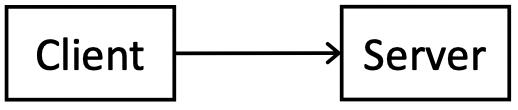
\includegraphics[width=1.5in]{OCPViolate}
					\end{minipage}
				\end{itemize}

			\begin{minipage}{0.5\textwidth}
			\item Conforming to the OCP\\
		\end{minipage}
			\begin{minipage}{0.5\textwidth}
				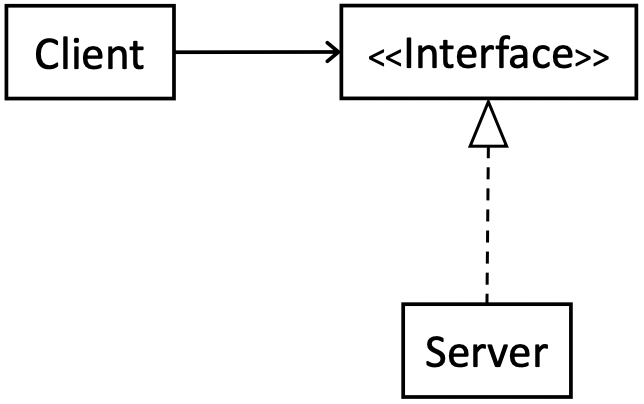
\includegraphics[width=0.4\textwidth]{OCPConform}
			\end{minipage}
		\end{itemize}

	\item The Liskov Substitution Principle (LSP)\\
		\textbf{\emph{Subtypes must be substitutable for their base types.}}
		\begin{itemize}
			\item Formally: Let $ \Phi(x) $ be a property provable about objects $ x $ of type $ T $. Then $ \Phi(y) $ should be true for objects $ y $ of type $ S $ where $ S $ is a subtype of $ T $.
			\item Counter-example: ``If it looks like a duck, quacks like a duck, but needs batteries – you probably have the wrong abstraction"
			\item Violating the LSP\\
				Issues\\
				\begin{minipage}{0.6\textwidth}
					\begin{itemize}
						\item Inheriting \textbf{height} and \textbf{width}
						\item Overriding \textbf{setHeight} and \textbf{setWidth}
						\item Conflicting assumptions. For example:
\begin{Verbatim}
void testRectangleArea(Rectangle r){
	r.setWidth(5);
	r.setHeight(4);
	assertEquals(r.computeArea(), 20);
}
\end{Verbatim}
					\end{itemize}
				\end{minipage}
				\begin{minipage}{0.3\textwidth}
					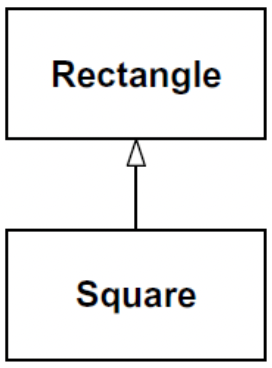
\includegraphics[width=1in]{LSPExample}
				\end{minipage}

			\item Implication: A model, viewed in isolation, cannot be meaningfully validated.
				\begin{itemize}
					\item The validity of a model can only be expressed in terms of its clients.
					\item One must view the design in terms of the reasonable assumptions made by
					the users of that design.
				\end{itemize}
		\end{itemize}

	\item The Interface Segregation Principle (ISP)\\
		\textbf{\emph{Clients should not be forced to depend on methods that they do not use.}}
		\begin{itemize}
			\item This principle deals with classes whose interfaces are not cohesive. That is, the interfaces of the class can be broken up into groups of methods where each group serves a different set of clients.
			\item When clients are forced to depend on methods that they don’t use, then those clients are subject to changes to those methods.\\
			\begin{minipage}[t]{0.4\textwidth}
				\item Violating the ISP\\
				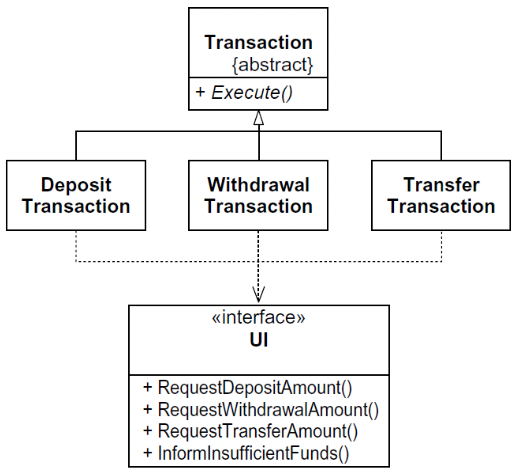
\includegraphics[width=2.5in]{ISPViolation}
			\end{minipage}
			\begin{minipage}[t]{0.6\textwidth}
				\item Conforming to the ISP\\
				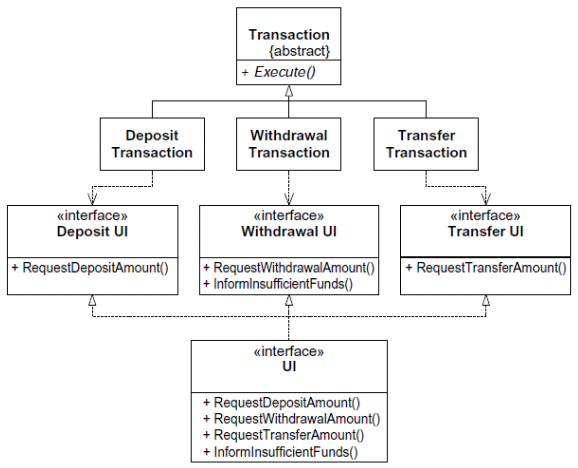
\includegraphics[width=3.5in]{ISPObey}
			\end{minipage}
		\end{itemize}

	\newpage

	\item The Dependency-Inversion Principle (DIP)
	\begin{enumerate}
		\item[\textbf{\textit{A.}}]  \textbf{\textit{High-level modules should not depend on low-level modules. Both should depend on abstractions.}}
		\item[\textbf{\textit{B.}}] \textbf{\textit{Abstractions should not depend on details. Details should depend on abstractions.}}
	\end{enumerate}
		\begin{itemize}
			\item The modules that contain the high-level business rules should take precedence over, and be independent of, the modules that contain the implementation details.
			\item When high-level modules depend on low-level modules, it becomes very difficult to reuse those high-level modules in different contexts.\\
			\begin{minipage}[t]{0.3\textwidth}
				\begin{center}
					\underline{\textbf{Naïve Layering}}\\
					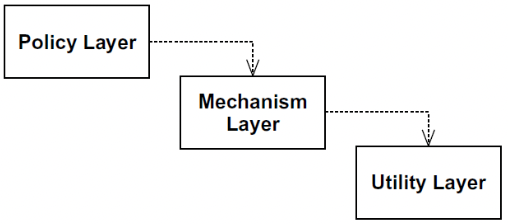
\includegraphics[width=2in]{DIPNaive}
				\end{center}
			\end{minipage}
			\begin{minipage}[t]{0.5\textwidth}
				\begin{center}
					\underline{\textbf{Inverted Layers}}\\
					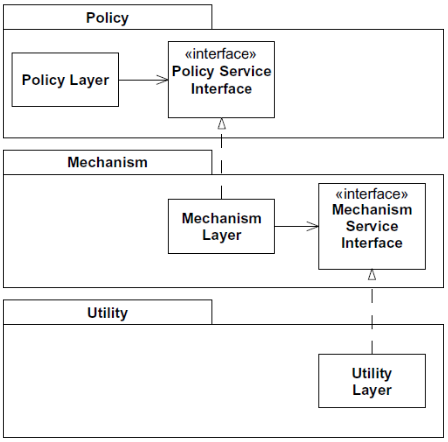
\includegraphics[width=2.5in]{DIPInverted}
				\end{center}
			\end{minipage}
		\\[10pt]
			\begin{minipage}[t]{0.5\textwidth}
				\item Violating the DIP\\
				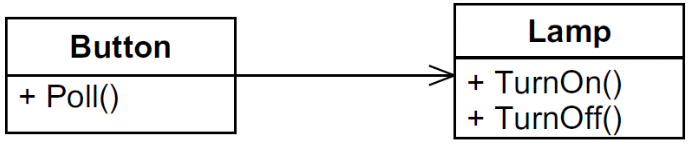
\includegraphics[width=2in]{DIPViolate}
			\end{minipage}
			\begin{minipage}[t]{0.5\textwidth}
				\item Conforming to the DIP\\
				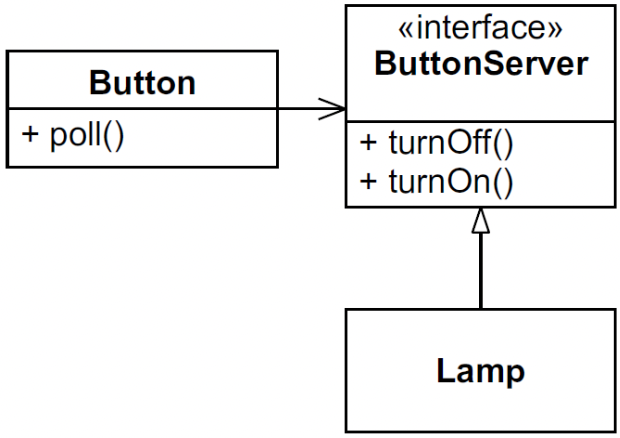
\includegraphics[width=2in]{DIPConform}
			\end{minipage}
		\end{itemize}

	\item Design Smells
		\begin{itemize}
			\item Symptoms of poor design
			\item Often caused by the violation of one or more of the design principles
				\begin{itemize}
					\item For example, the smell of \textit{Rigidity} is often a result of insufficient attention to OCP.
				\end{itemize}
			\item These symptoms include:
				\begin{enumerate}
					\item Rigidity -- The design is hard to change.
					\item Fragility -- The design is easy to break.
					\item Immobility -- The design is hard to reuse.
					\item Viscosity -- It is hard to do the right thing.
					\item Needless Complexity -- Overdesign.
					\item Needless Repetition -- Mouse abuse.
					\item Opacity -- Disorganized expression.
				\end{enumerate}
		\end{itemize}
\end{itemize}

\newpage

\section{Software Development Life Cycle}
	\begin{itemize}
		\begin{minipage}{0.65\textwidth}
			\item Software Development Life Cycle (SDLC)
				\begin{itemize}
					\item \textbf{Planning} -- develop a plan for creating the concept or evolution of the concept
					\item \textbf{Analysis} -- analyze the needs of those using the system. Create detailed requirements
					\item \textbf{Design} -- Translate the detailed requirements into detailed design work
					\item \textbf{Implementation} -- Complete the work of developing and testing the system
					\item \textbf{Maintenance} -- Complete any required maintenance to keep the system running
				\end{itemize}
		\end{minipage}
		\begin{minipage}{0.02\textwidth}
		\end{minipage}
		\begin{minipage}{0.33\textwidth}
			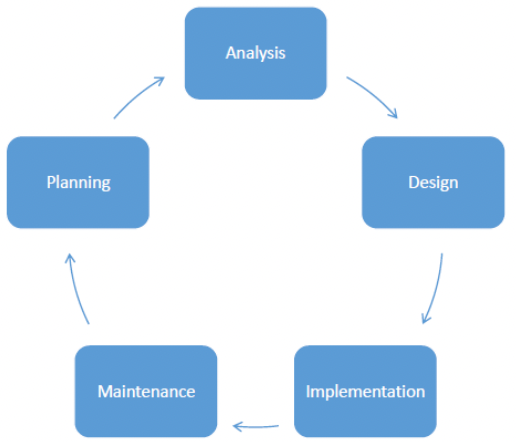
\includegraphics[scale=0.7]{SDLCCircle}
		\end{minipage}

		\item Different SDLC implementations
			\begin{itemize}
				\item Rigid timeline / budget (Waterfall)
				\item Rick Adverse (Spiral)
				\item Quality Deliverables / Less management (Agile)
			\end{itemize}

		\item Waterfall
			\begin{itemize}
				\item A sequential (non-iterative) model
				\item Involves a large amount of upfront work, in an attempt to
				reduce the amount of work done in later phases of the project
			\end{itemize}
			\begin{center}
				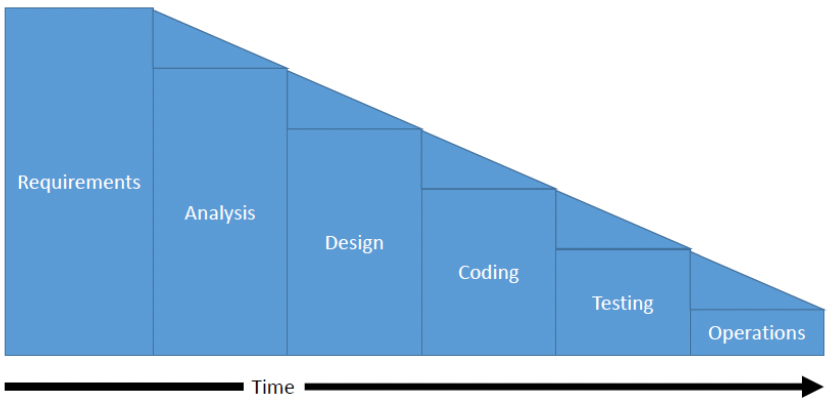
\includegraphics[scale=0.5]{Waterfall}
			\end{center}

		\item Spiral\\
			\begin{minipage}{0.7\textwidth}
				\begin{itemize}
					\item Risk-driven model
					\item More time is spent on a given phase based on the amount of risk that phase poses for the project
				\end{itemize}
			\end{minipage}
			\begin{minipage}{0.3\textwidth}
				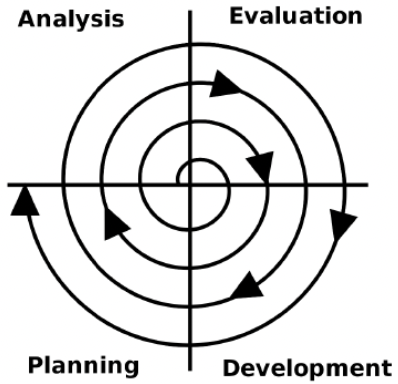
\includegraphics[scale=0.5]{Spiral}
			\end{minipage}

		\item Agile
			\begin{itemize}
				\item Issues with Waterfall
					\begin{itemize}
						\item Inappropriate when requirements change frequently
						\item Time gets squeezed the further into the process you get
					\end{itemize}
				\item Agile Methodologies
					\begin{itemize}
						\item Extreme Programming (XP)
						\item Scrum
						\item Test-driven Develpoment (TDD)
						\item Feature-driven Development (FDD)
						\item Etc.
					\end{itemize}
			\end{itemize}

		\item Agile Manifesto\\
			\emph{``We are uncovering better ways of developing software by doing it and helping others do it. Through this work, we have come to value:\\
				\hspace*{10mm} \textbf{Individuals and interactions} over processes and tools\\
				\hspace*{10mm} \textbf{Working software} over comprehensive documentation\\
				\hspace*{10mm} \textbf{Customer collaboration} over contract negotiation\\
				\hspace*{10mm} \textbf{Reponding to change} over following a plan\\
			That is, while there is value in the items on the right, we value the items on the left more."}

		\item Agile vs. Waterfall\\
			\begin{tabular}{| r c c |}
				\hline
				 & \textbf{Agile} & \textbf{Waterfall}\\
				 Iterative? & \cellcolor{green!25}Yes & \cellcolor{green!15}No\\
				 Late changes? & \cellcolor{green!25}Yes & \cellcolor{green!15}No / \$\$\$\\
				 Fixed timeline? & \cellcolor{green!15}No* & \cellcolor{green!25}Yes\\
				 Fixed cost? & \cellcolor{green!15}No* & \cellcolor{green!25}Yes*\\
				 Volume of meetings & \cellcolor{green!25}Consistent & Heavy up front, reduced middle, heavy end\\
				 Release frequency & \cellcolor{green!25}Every sprint & \cellcolor{green!15}Once per project\\
				 Business Involvement & Heavy throughout & Heavy early, and at very end\\
				 Cost to fix mistakes & \cellcolor{green!25}Low & \cellcolor{green!15}High\\
				 \hline
			\end{tabular}

		\item eXtreme Programming (XP)
			\begin{itemize}
				\item One of the most rigorous forms of Agile
				\item Involves building a series of feedback loops, which are used to help guide when change can occur and allow for changes to be quickly integrated into the plan for development
				\item Built on the idea that you can reduce the cost of developing software, and build better software, by having goals
				\item XP requires that everything that can be unit tested is unit tested, that everyone works in pairs, and that these pairs change frequently
			\end{itemize}

		\item Code Review
			\begin{itemize}
				\item Although pair programming has gone out of vogue along with XP, it is important to note a practice that has become common place that was born from this idea -- Code Review.
				\item A code review is a session in which you \textbf{must sit down with another developer} from the team and walk them through your implementation line-by-line in order to get advice and feedback.
				\item This process has been shown to lead to better code, through finding bugs earlier, and an increased amount of collaboration on difficult concepts.
			\end{itemize}

		\item Scrum
			\begin{itemize}
				\item Scrum is currently one of the most widely used methodologies of software development\\[-15pt]
			\end{itemize}
			\begin{center}
				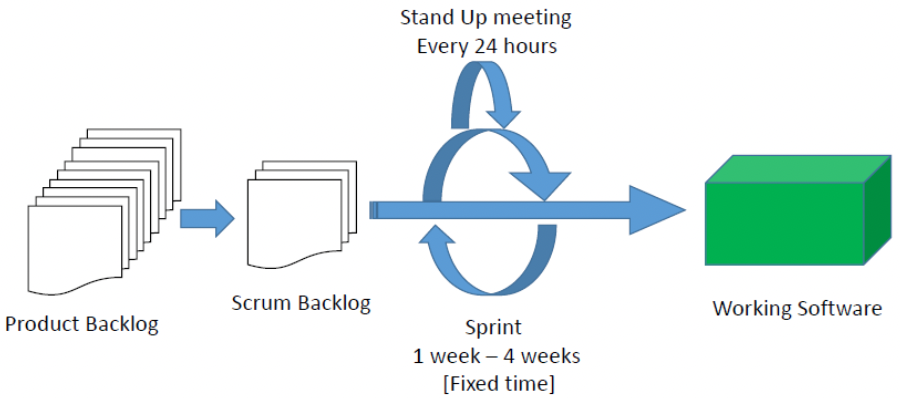
\includegraphics[scale=0.5]{Scrum}
			\end{center}

		\item Scrum - Roles
			\begin{itemize}
				\item Product Owner
					\begin{itemize}
						\item Responsible for delivering requirements and accepting demos
						\item Involved in planning session
					\end{itemize}
				\item Scrum Master
					\begin{itemize}
						\item Responsible for removing impediments
					\end{itemize}
				\item Team members
					\begin{itemize}
						\item No one has a fixed role other than the scrum master and product owner
						\item Everyone takes on tasks, and completes them based on what they are most comfortable with
					\end{itemize}
			\end{itemize}

		\item Scrum - Sprint
			\begin{itemize}
				\item The sprint is a fixed time to deliver a working set of features, that are reviewed in a demonstration to the product owner
				\item Tasks in Scrum are broken into “User Stories”
				\item In a sprint, a team agrees at the beginning to take on a certain
				number of user stories
				\item Sprints are usually between 1 and 4 weeks in length
				\item At the end of each sprint, teams hold a “retrospective” which is a meeting where the past sprint is discussed, and chances for improvement for the next sprint are raised
			\end{itemize}

		\item Scrum - User Stories
			\begin{itemize}
				\item User stories are similar to requirements. They are written in the following format:\\
					\hspace*{10mm}\emph{As a \{ACTOR/OBJECT\} I want to \{ACTION\} so that \{RESULT\}}
			\end{itemize}

		\item Scrum - Planning Poker
			\begin{itemize}
				\item In scrum, we do not assign time to tasks, but assign arbitrary points. This is a form of estimation that helps gauge how much work something will take to complete.
				\item Planning poker takes a set of pre-determined numbers (usually: 1, 2, 3, 5, 8, etc.) and gets you to estimate how much work something will be relative to a known task.
				\item After discussing the story at hand , everyone selects a card. Then, the cards are turned over simultaneously. Usually time is given for those who had the lowest and highest numbers to state their case
				\item The process is repeated until everyone ends up at the same number.
			\end{itemize}

		\item Scrum - Planning Session
			\begin{itemize}
				\item Planning sessions happen at the start of each sprint.
				\item They usually take a few hours. During this time, the team decides how much work it will take on, and discusses any major technical challenges they expect to face.
				\item Usually, Product Owners are available for at least a portion of this meeting, to help with prioritization. They are only there to assist in this regard, and not to dictate what the team will complete.
			\end{itemize}

		\item Scrum - The Standup Meeting
			\begin{itemize}
				\item Happens EVERY SINGLE day that you are working
				\item The goal is to make sure people are doing alright
				\item Shouldn’t be longer than 15 minutes
				\item Answer three questions:
					\begin{enumerate}
						\item What did I finish since the last standup?
						\item What am I going to finish by the next standup?
						\item What is stopping me / what impediments am I facing?
					\end{enumerate}
			\end{itemize}

		\item Scrum - Working Agreement
			\begin{itemize}
				\item A series of statements that everyone on the team agrees to about how the team will work
				\item Things in working agreements may include:
					\begin{itemize}
						\item The standup will occur at 1:00 pm every day, and last 15 minutes
						\item We will not speak during the standup, unless it is our turn to speak
						\item Our meetings will take place in the lobby of the IC building
						\item All code must be peer-reviewed
						\item We will submit all code 24 hours prior to the due date
					\end{itemize}
			\end{itemize}

		\item Scrum - Definition of Done
			\begin{itemize}
				\item A formal agreement of when work is considered complete
				\item For example, a story can be marked as done when:
					\begin{itemize}
						\item It has been fully unit tested
						\item It successfully integrated with the rest of the code
						\item It has been peer reviewed
						\item It is fully commented
						\item Etc.
					\end{itemize}
				\item It is important that team comes to an agreement on this definition before they start work.
			\end{itemize}

		\item Test Driven Development (TDD)
			\begin{itemize}
				\item TDD is a way to develop software that revolves around writing test cases.
				\item The basic concept is to write the unit tests needed to be passed for a feature to be considered working. You then code to the unit tests –writing the minimum amount for the tests to succeed.
				\item Once working, you review and refactor. Then move on to the next set of tests.\\[-15pt]
				\begin{center}
					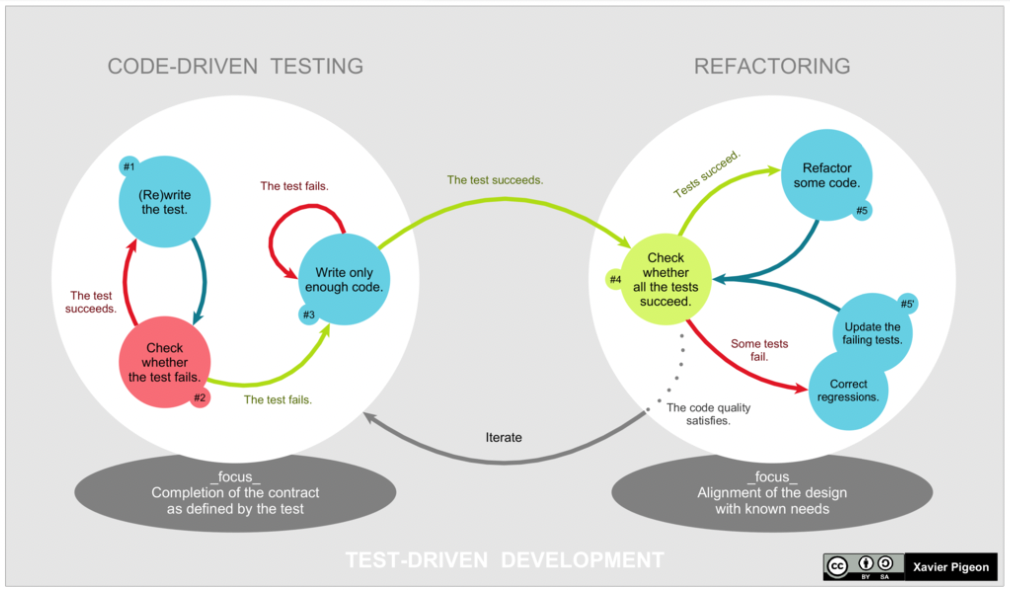
\includegraphics[scale=0.8]{TDD}
				\end{center}
			\end{itemize}

		\item Feature Driven Development (FDD)
			\begin{itemize}
				\item Based on the idea of building a focused model for the project, and the iterating on the features needed.
				\item Splits development into 5 major pieces:
					\begin{enumerate}
						\item Develop overall model
						\item Build feature list
						\item Plan by feature
						\item Design by feature
						\item Build by feature
					\end{enumerate}
			\end{itemize}

	\end{itemize}

\newpage

\section{I/O and Regular Expressions}

\begin{itemize}
	\item Input and Output (I/O)
		\begin{itemize}
			\begin{minipage}[t]{0.3\textwidth}
				\item Input sources include:
				\begin{itemize}
					\item Keyboard
					\item File
					\item Network
				\end{itemize}
			\end{minipage}
			\begin{minipage}[t]{0.5\textwidth}
			\item Output destinations include:
				\begin{itemize}
					\item Console
					\item File
					\item Network
				\end{itemize}
			\end{minipage}
		\end{itemize}

	\item Input and Output Streams
		\begin{itemize}
			\item Java handles inputs and outputs using streams\\
			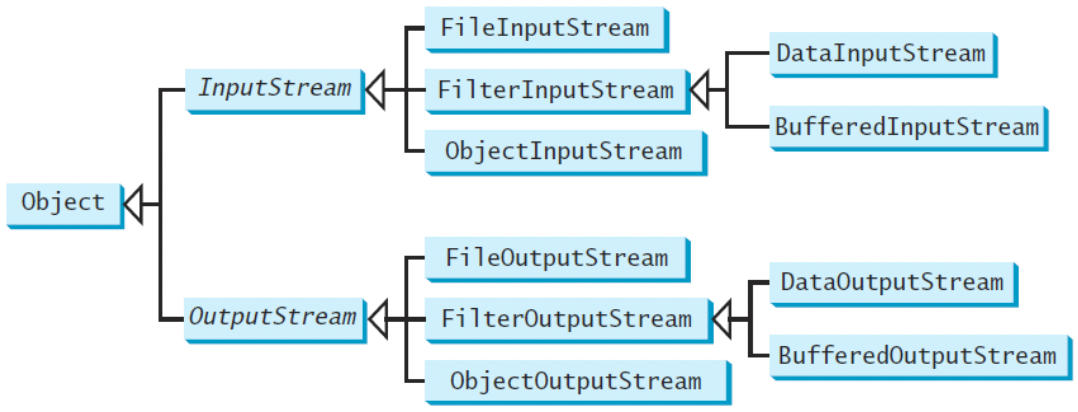
\includegraphics[scale=0.6]{IOChart}
		\end{itemize}

	\item Standard I/O
		\begin{itemize}
			\item \textbf{System.in}
				\begin{itemize}
					\item Object of type \textbf{InputStream}
					\item Typically refers to the keyboard
					\item Reading data could be done using the \textbf{Scanner} class. Its methods include:
						\begin{itemize}
							\begin{minipage}{0.2\textwidth}
								\item \textbf{String next()}
								\item \textbf{String nextLine()}
							\end{minipage}
							\begin{minipage}{0.4\textwidth}
								\item \textbf{int nextInt()}
								\item \textbf{double nextDouble()}
							\end{minipage}
						\end{itemize}
				\end{itemize}

			\item \textbf{System.out}
				\begin{itemize}
					\item Object of type \textbf{PrintStream}
					\item Typically refers to the console
				\end{itemize}
		\end{itemize}

	\item The \textbf{File} class
		\begin{itemize}
			\item Contains methods for obtaining the properties of a file/directory and
			for renaming and deleting a file/directory
			\item Files could be specified using absolute or relative names
			\item Constructing a \textbf{File} instance does not create a file on the machine
			\item Methods include:
				\begin{itemize}
					\begin{minipage}[t]{0.3\textwidth}
						\item \textbf{boolean createNewFile()}
						\item \textbf{boolean delete()}
						\item \textbf{boolean exists()}
					\end{minipage}
					\begin{minipage}[t]{0.5\textwidth}
						\item \textbf{boolean isDirectory()}
						\item \textbf{File [] listFiles()}
					\end{minipage}
				\end{itemize}
		\end{itemize}

	\item File I/O
		\begin{itemize}
			\item Reading could be done using the \textbf{Scanner} class
				\begin{itemize}
					\item e.g. \textbf{Scanner input = new Scanner(new File(filename));}
				\end{itemize}
			\item Writing could be done using the \textbf{FileWrite} class
				\begin{itemize}
					\item e.g. \textbf{FileWriter output = new FileWriter(filename, append);}
				\end{itemize}
		\end{itemize}

	\newpage

	\item Regular Expressions
		\begin{itemize}
			\item A regular expression (abbreviated regex) is a string that describes a pattern for matching a set of strings.
			\item Regular expressions provide a simple and effective way to validate user input
				\begin{itemize}
					\item e.g. phone numbers
				\end{itemize}
			\item Java supports regular expressions using the \textbf{java.util.regex} package
			\item The \textbf{Pattern} class can be used to define the pattern
				\begin{itemize}
					\item The \textbf{compile} method takes a string representing the regular expression as an argument and compiles it into a pattern
				\end{itemize}
			\item The \textbf{Matcher} class can be used to search for the pattern. Its methods include:
				\begin{itemize}
					\item \textbf{boolean find()}
					\item \textbf{boolean matches()}
				\end{itemize}
			\item Example
			\begin{Verbatim}
	Pattern pattern = Pattern.compile("H.*d");
	Matcher matcher = pattern.matcher("Hello World");
	System.out.println(matcher.matches());
			\end{Verbatim}
		\end{itemize}

	\item Commonly Used Regular Expressions\\
		\begin{tabular}{l l l}
			\hline
			\textit{Regular Expression} & \textit{Matches} & \textit{Example}\\
			\hline
			\hline
			\texttt{.} & any single character & \texttt{Java} matches \texttt{J..a}\\
			\texttt{(ab|cd)} & \texttt{ab} or \texttt{cd} & \texttt{ten} matches \texttt{t(en|im)}\\
			\texttt{[abc]} & \texttt{a}, \texttt{b}, or \texttt{c} & \texttt{Java} matches \texttt{Ja[uvwx]a}\\
			\texttt{[\string^abc]} & any character except \texttt{a}, \texttt{b}, or \texttt{c} & \texttt{Java} matched \texttt{Ja[\string^ars]a}\\
			\texttt{[a-z]} & \texttt{a} through \texttt{z} & \texttt{Java} matches \texttt{[A-M]av[a-d]}\\
			\texttt{[\string^a-z]} & any character except \texttt{a} through \texttt{z} & \texttt{Java} matches \texttt{J]av[\string^b-d]}\\
			\texttt{[a-e[m-p]]} & \texttt{a} through \texttt{e} or \texttt{m} through \texttt{p} & \texttt{Java} matches \texttt{[A-G[I-M]]av[a-d]}\\
			\texttt{[a-e\&\&[c-p]] }& intersection of \texttt{a-e} with \texttt{c-p} & \texttt{Java} matches \texttt{[A-P\&\&[I-M]]av[a-d]}\\
			\texttt{\textbackslash d} & a digit, same as \texttt{[0-9]} & \texttt{Java2} matches ``\texttt{Java[\textbackslash\textbackslash d]}'' \\
			\texttt{\textbackslash D} & a non-digit & \texttt{\$Java} matches ``\texttt{[\textbackslash\textbackslash D][\textbackslash\textbackslash D]ava}"\\
			\texttt{\textbackslash w} & a word character & \texttt{Java1} matches ``\texttt{[\textbackslash\textbackslash w]ava[\textbackslash\textbackslash w]}"\\
			\texttt{\textbackslash W} & a non-word character & \texttt{\$Java } matches ``\texttt{[\textbackslash\textbackslash W][\textbackslash\textbackslash w]ava}"\\
			\texttt{\textbackslash s} & a whitespace character & ``\texttt{Java 2}'' matches ``\texttt{Java\textbackslash\textbackslash s2}"\\
			\texttt{\textbackslash S} & a non-whitespace character & \texttt{Java} matches ``\texttt{[\textbackslash\textbackslash S]ava}"\\
			\hline
			\texttt{\emph{p*}} & zero or more occurrences of pattern \texttt{\emph{p}} & \makecell[cc]{\texttt{aaaabb} matches ``\texttt{a*bb}" \\ \texttt{ababab} matches ``\texttt{(ab)*}"}\\
			\hline
			\texttt{\emph{p+}} & one or more occurrences of pattern \texttt{\emph{p}} & \makecell[cc]{\texttt{a} matches ``\texttt{a+b*}" \\ \texttt{able} matches ``\texttt{(ab)+.*}"}\\
			\hline
			\texttt{\emph{p?}} & zero or one occurrence of pattern \texttt{\emph{p}} & \makecell[cc]{\texttt{Java} matches ``\texttt{J?Java}" \\ \texttt{Java} matches ``\texttt{J?ava}"}\\
			\hline
			\texttt{\emph{p\{n\}}} & exactly \texttt{n} occurrences of pattern \texttt{\emph{p}} & \makecell[cc]{\texttt{Java} matches ``\texttt{J\{1\}.*}" \\ \texttt{Java} does not match ``\texttt{.\{2\}}"}\\
			\hline
			\texttt{\emph{p\{n,\}}} & at least \texttt{n} occurrences of pattern \texttt{\emph{p}} & \makecell[cc]{\texttt{aaaa} matches ``\texttt{a\{1,\}}" \\ \texttt{a} does not match ``\texttt{a\{2,\}}"}\\
			\hline
			\texttt{\emph{p\{n, m\}}} & between \texttt{n} and \texttt{m} occurrences (inclusive) & \makecell[cc]{\texttt{aaaa} matches ``\texttt{a\{1,9\}}" \\ \texttt{abb} does not match ``\texttt{a\{2,9\}bb}"}\\
		\end{tabular}

\end{itemize}

\end{document}